\section{Analysis}\label{analysis}
%The next line produces an indented paragraph to start the document
 %unit.  The LaTeX defaults start most units without indentations.
\hspace{\parindent}
Outline the analysis section.

%%%%%%%%%%%%%%%%%%%%%%%%%%%%%%%%%%%%%%%%%%%%%%%%%%%%%%%%%%%
% Particle Identification and Event Selection
%%%%%%%%%%%%%%%%%%%%%%%%%%%%%%%%%%%%%%%%%%%%%%%%%%%%%%%%%%%
\subsection{Particle Identification and Event Selection}
  After the particle tracks are reconstructed, we use a predictive model to
  classify proton tracks. The inputs to the model are the reconstructed
  physical variables, and the output is the probability that the track is from
  a proton vs. some other particle. There are many predictive models that we
  can use, each with advantages and disadvantages. We chose gradient-boosted
  decision trees for a few main reasons: they are easily interpretable, the
  inputs can be a mix of numeric and categorical variables, and boosted
  decision trees perform well at identifying a small signal in a large
  background.  Each tree is essentially a series of cuts based on physical
  variables which have been fine-tuned to increase the efficiency and purity of
  the final selected sample.
  \subsubsection{Reconstructed track features}
    The reconstructed features that are used as input to the classifier are
    listed below. Most of the features come directly from the track object, but
    some are created for this classifier. Each of the features used to identify
    protons either helps to separate neutrino-induced tracks from
    cosmic-induced tracks or to separate neutrino-induced proton tracks from
    other neutrino-induced particle types.

    First is a list and description of the features designed to separate
    neutrino-induced protons from other neutrino-induced particle types.
    \begin{itemize}
      \item \textbf{Number of hits:} This is the total number of hits on all
      three wire planes associated with track. When used in combination with
      track length and average energy deposited, this feature can be used to
      determine the hit and energy density of the track.
      \item \textbf{Straightness:} This is the ratio of distance between
      reconstructed end points (displacement) to reconstructed path length. It
      represents the amount of scattering a track undergoes. The value is
      always betwen zero and one with one being perfectly straight.
      \item \textbf{Cosmic score:} This is the geometry tagging cosmic score
      from Sec.~\ref{sec:tpcreco}. Tracks with a cosmic score of 1 have already
      been removed in the cosmic hit removal stage. So, this value is either 0
      (fully contained within the TPC) or 0.5 (entering or exiting the TPC).
      \item \textbf{Particle ID from energy deposited per unit length (dE/dx):}
      The PIDA and $\chi^2$ PID algorithms values described in
      Sec.~\ref{sec:tpcreco} are used.
      \item \textbf{Length:} This is the reconstructed 3D track length found by
      stepping along the trajectory points.
      \item \textbf{Start and end dQ/dx:} These are the total charge deposited
      at start and end points of track divided by the distance between hits to
      account for the angle with respect to the wires. The total charge of the
      first (or last) six track hits on each plane is summed.
      \item \textbf{End to start dQ/dx ratio and difference:} These are the
      ratio and difference of the end dQ/dx divided by (or subtracted by) the
      start dQ/dx described in the previous item.
      \item \textbf{Total dQ/dx:} This is the sum of the dQ/dx of all hits on
      all planes associated with track.
      \item \textbf{Average dQ/dx:} This is the total dQ/dx divided by the
      number of hits associated with track.
    \end{itemize}

    Next is the list and description of the features designed to separate
    neutrino-induced tracks from cosmic-induced tracks.
    \begin{itemize}
      \item \textbf{Start and end positions:} These are the reconstructed x, y,
      and z positions of start and end of the track. Tracks that start closer
      to a TPC boundary are more likely to be cosmic-induced.
      \item \textbf{$\theta$ and $\phi$:} These are the reconstructed polar and
      azimuthal angles with respect to the beam direction. Vertical tracks are
      much more likely to be cosmic-induced, while forward-going tracks are
      more likely to be from the neutrino beam.
    \end{itemize}
   
    Determining which end of a track is the beginning is difficult when a
    vertex is not observable. Since we are particularly interested in
    neutral-current elastic events with only a single proton, the direction of
    the track is a concern. A proton will deposit much more energy at the end
    of its track than at the beginning which can be used to determine the true
    direction. Since this correction is not currently implemented in pandoraNu,
    we take all reconstructed tracks that have a higher start charge than end
    charge and flip them. This means changing the saved start positions, end
    positions, $\theta$, $\phi$, start dQ/dx, end dQ/dx, and the end to start
    dQ/dx ratio and difference.
    
  \subsubsection{Boosted decision trees}\label{sec:decisiontrees}
    A decision tree can be thought of as a series of if/else statements that
    separate a data set into two or more classes as illustrated in
    Fig.~\ref{fig:dtree}. At each node of the tree, a split is chosen to
    maximize information gain until a set level of separation is reached.  At
    the terminus of the series of splits, called a leaf, a class is assigned.
    The usual parameters that can be set when creating a decision tree are: the
    maximum depth of the tree (how many layers of nodes you will allow), the
    minimum split size (how many data points do you require to keep splitting),
    and minimum leaf size (how small does a leaf have to be before you stop). 
    \begin{figure}[ht]
      \centering
      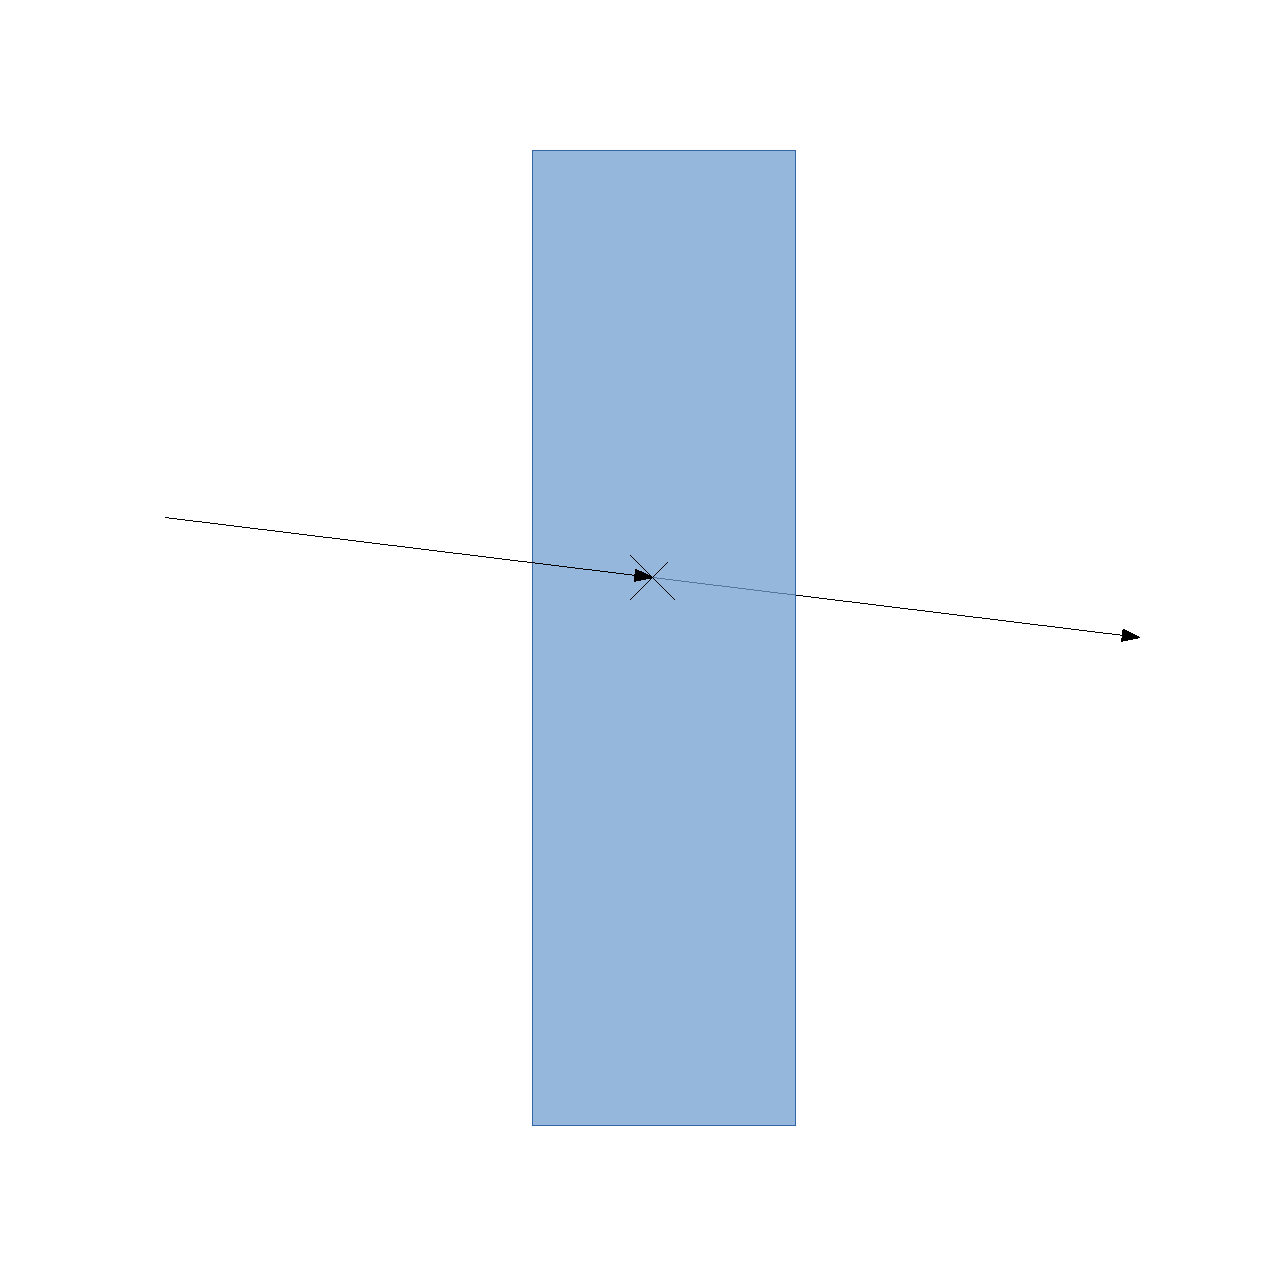
\includegraphics[angle=0,width=4in]{figures/bz.pdf}
      \caption{Graphical example of a decision tree.}
      \label{fig:dtree}
    \end{figure}
    
    A single tree can easily overfit a data set if it is at all complex, and
    its output is just a class label. Gradient-boosting addresses both of these
    issues by combining many weak classifiers into a strong one. Each weak
    classifier is built based on the error of the previous one. For a given
    training set, whenever a sample is classified incorrectly by a tree, that
    sample is given a higher importance when the next tree is being created.
    Mathematically, each tree is training on the gradient of the loss function.
    After all of the trees have been created, each tree is given a weight based
    on its ability to classify the training set, and the output of the
    gradient-boosted decision tree classifier is the probability that a sample
    is in a given class.
    
    The gradient-boosted decision tree software package we use is
    XGBoost~\cite{xgboost}. There are two types of classifiers we can use to
    separate protons from other tracks: binary and multiclass. Both classifiers
    are trained on all types of reconstructed tracks. A binary classifier
    classifies each track as either a proton or not a proton, and a multiclass
    classifier classifies a track as one of many types including a proton. We
    choose to use multiclass because the information about non-proton tracks is
    useful for event identification. The five classes that we train the
    decision trees to classify are protons (both BNB and cosmic), BNB muons,
    BNB pions, BNB electrons/photons, and all non-proton cosmics.
    
    The decision trees were trained to select protons in general. The target
    class contains all protons from BNB interactions, as well as cosmic
    protons. However, the choice of track features and most of the improvements
    that were made were done with the goal of a high efficiency for isolated
    protons and cosmic rejection.

  \subsubsection{Training}
    Describe the training sets. What samples were used, how many of everything,
    and all hyperparamter settings. Describe hyperparameter optimization. 
  \subsubsection{Performance}
    Show efficiency, accuracy, itemize backgrounds.
    Discuss reasons for different backgrounds.
  \subsubsection{Event selection}
    Need to select both NCE and CCQE events.
    Use particle ID plus reconstructed flashes.
    Exactly how we select NCE events 

%%%%%%%%%%%%%%%%%%%%%%%%%%%%%%%%%%%%%%%%%%%%%%%%%%%%%%%%%%%
% Efficiency and Background Estimation
%%%%%%%%%%%%%%%%%%%%%%%%%%%%%%%%%%%%%%%%%%%%%%%%%%%%%%%%%%%
\subsection{Efficiency and Background Estimation}\label{background}
  \subsubsection{Event selection efficiency}
    Efficiency due to TPC, PMT software trigger, reconstruction, proton ID,
    event selection, etc. This includes efficiency due to proton reinteracting
    in the nucleus and other nuclear effects.
  \subsubsection{Beam Induced Dirt Background}
    Discuss dirt neutrons, how they happen and estimated rates and energy
    distributions.  Show how well we can seperate or understand them. Show any
    sort of data-driven correction we did to dirt neutron background and how it
    affects our uncertainty. Talk about how well we can tag cryostat neutrons
    with the PMTs.
  \subsubsection{Beam Induced TPC Background}
    Talk about neutral-current elastic neutrons that are produced in the TPC
    and how their distributions differ from NCEp ones. Also include BNB
    backgounds (CCQE where muon wasn't reconstructed, NCpi0, etc.) Discuss how
    the optical signal would be different for each of these.
  \subsubsection{Cosmic Background}
    Discuss the difference between cosmic tracks and beam proton tracks. How do
    we separate them? What is the rate?

%%%%%%%%%%%%%%%%%%%%%%%%%%%%%%%%%%%%%%%%%%%%%%%%%%%%%%%%%%%
% Ratio of Cross Sections
%%%%%%%%%%%%%%%%%%%%%%%%%%%%%%%%%%%%%%%%%%%%%%%%%%%%%%%%%%%
\subsection{Ratio of NCEp to CCQEn Cross Sections}\label{sec:ratios}
  Show how the ratio gets rid of a lot of measurement uncertainty like beam
  flux and efficiencies. Give exact equation that we will be using for
  analysis. Show how $\Delta s$ is still large at low $Q^2$.
  \subsubsection{Sources of Measurement Uncertainty}
    TPC efficiency: If ionization electrons actually reach the
    TPC and leave a signal.
    PMT trigger efficiency: Refer back to PMT trigger studies. Give uncertainty
    due to on signal.
    Reconstruction efficiency: Refer back. Give uncertainty on signal.
  \subsubsection{Quantifying Uncertainty on Ratio}\label{errorcalc}
    Calculate exact uncertainty and show it here.
  \subsubsection{Model uncertainty}\label{sec:modeluncertainty}
    Nuclear effects and FSI. Discuss. Discuss which values are varied and by
    how much? Refer to reweighting section. 

%%%%%%%%%%%%%%%%%%%%%%%%%%%%%%%%%%%%%%%%%%%%%%%%%%%%%%%%%%%
% Comparison to Simulation
%%%%%%%%%%%%%%%%%%%%%%%%%%%%%%%%%%%%%%%%%%%%%%%%%%%%%%%%%%%
\subsection{Comparison of data to simulation}
  To determine what true physics values would have caused the data that we
  measure, we need to compare the data to Monte Carlo simulation. The physics
  model is a combination of many different physics models including nuclear
  physics models, neutrino cross section models, nucleon structure models,
  cosmic ray models, and others. It is too complicated to calculate the
  parameters directly. Instead, we simulate what data we would see in the
  detector given a set of physical parameters and models, and compare that
  directly to the actual data we detected. We do this for many possible values
  of the parameters and calculate the likelihood for each set of values. In
  addition to varying the parameters that we want to measure in the simulation,
  we vary the physical parameters whose true values aren't well constrained
  which might have a large effect on the final data. This allows us to quantify
  the uncertainty due to unknown quantities.
  \subsubsection{Event reweighting}\label{sec:reweighting}
    Full Monte Carlo simulations are both time and computing intensive. Instead
    of re-running the simulation for each possible parameter value that we are
    interested in, we can calculate the ratio of the probabilities of each
    interaction occurring given the new values to the probabilities of each
    interaction occurring for the original simulated parameter values. We refer
    to this ratio as an event weight:
    \begin{equation}
      w = \frac{P(\textrm{event}|\theta')}{P(\textrm{event}|\theta)} \,,
    \end{equation}
    where $w$ is the event weight for a given event, $P($event$|\theta)$ is the
    probability of the simulated event given the set of original parameters
    used in the simulation, $\theta$, and $P($event$|\theta')$ is the
    probability of the simulated event given a new set of parameters,
    $\theta'$.

    Since the four parts of GENIE cross section model (the nuclear physics
    model, the neutrino-nucleon cross section model, the hadron production
    model, and the intranuclear hadron transport model from
    Sec.~\ref{sec:geniexsec}) are treated independently in NC elastic
    events~\cite{GENIE}, the event weight, w, factors:
    \begin{equation}\label{eq:weights}
      w = w_{\textrm{nuclear}}\times w_{\textrm{neutrino-nucleon}}\times 
          w_{\textrm{hadron prod.}}\times w_{\textrm{intranuclear}} \,,
    \end{equation}
    where $w_{\textrm{nuclear}}$ is the nuclear physics model weight,
    $w_{\textrm{neutrino-nucleon}}$ is the neutrino-nucleon cross section model
    weight, $w_{\textrm{hadron prod.}}$ is the hadron production model weight,
    and $w_{\textrm{intranuclear}}$ is the intranuclear hadron transport model
    weight. So, only the NC elastic cross section probability ratio needs to be
    calculated to see the effect of $\Delta s$ or another cross section
    parameter of interest.

    The probability of a neutrino interaction is proportional to the
    interaction cross section, so the weight, $w_{\textrm{neutrino-nucleon}}$
    is just a ratio of cross sections
    \begin{equation}
      w_{\textrm{neutrino-nucleon}} = w_{\sigma} 
        = \frac{d^n\sigma'_{\nu}/dK^n}{d^n\sigma_{\nu}/dK^n} \,,
    \end{equation}
    where $d^n\sigma/dK^n$ is the differential cross section for the initially
    simulated neutrino-nucleon interaction, and $d^n\sigma'/dK^n$ is the
    differential cross section with the modified parameters evaluated at the
    kinematical phase space $\{K^n\}^3$. The differential cross section is a
    function of the neutrino energy in the rest frame of the scattered nucleon,
    $E_{\nu}^{(nRF)}$, the interaction four-momentum transfer, $Q^2$, and the
    physics model including parameters of the model.

    To determine the effect of the NC elastic axial form factor parameters
    $\Delta s$ and $M_A^s$ on the data, we calculate the NC elastic cross
    section given these new parameters and the cross section given the initial
    simulation parameters for each NC elastic event in the Monte Carlo
    simulation. To get an accurate weight, the denominator needs to be
    calculated exactly as the cross section was calculated in the initial
    GENIE. However, there is no reason that a different model can't be used for
    the numerator. For the numerator, we use the LLewellyn-Smith
    neutrino-nucleon elastic cross section parameterization described in
    Sec.~\ref{sec:nuxsec}. For the vector form factors, we use the
    Arrington-Sick model with two-photon exchange (TPE) described in
    Sec.~\ref{sec:vectorff}. For the NC axial form factor, $G_A^{NC}$, we use a
    modified dipole form. The up and down quark terms of the axial form factor,
    $G_A$, have the same form as the Ahrens et al.~\cite{Ahrens}
    parameterization with the parameter values used in the GENIE
    implementation. The strange quark term of the axial form factor, $G_A^s$,
    also has the Ahrens et al. parameterization, but the $M_A$ parameter value
    is allowed to be different than in the $G_A$ term. We call this new
    parameter $M_A^s$
    \begin{align}\label{eq:modifiedaxial}
      G_A^{NC}(Q^2) = \frac{1}{2}G_A(Q^2) - \frac{1}{2}G_A^s(Q^2) \,,& \\
      G_A(Q^2) = \frac{g_A}{(1+\frac{Q^2}{M_A})^2} \,,& \\
      G_A^s(Q^2) = \frac{\Delta s}{(1+\frac{Q^2}{M_A^s})^2} \,.&
    \end{align}
    Figure~\ref{fig:ncxseccompare} shows the effect on simulated NC elastic
    neutrino-proton events due to the updated cross section model,
    $\left(\frac{d\sigma}{dQ^2}\right)$. In the comparison the cross section
    parameterization is changed, but the parameter values are the same as the
    ones used in the GENIE, $\left(\frac{d\sigma}{dQ^2}\right)_{GN}$,
    parameterization wherever applicable.
    \begin{figure}[ht]
      \centering
      \begin{subfigure}[t]{2.5in}
        \includegraphics[angle=0,width=2.5in]{figures/analysis/comparison/NCxsec_Compare.png}
        \caption{The X-axis is the value of the NC elastic cross section used
        in GENIE for each simulated event, and the Y-axis is the value of the
        NC elastic cross section used in this analysis for the same given
        event.}
      \end{subfigure}
      \hspace{2pt}
      \begin{subfigure}[t]{2.5in}
        \includegraphics[angle=0,width=2.5in]{figures/analysis/comparison/NCxsec_Compare_Difference.png}
        \caption{The X-axis is the value of the NC elastic cross section used
        in GENIE for each simulated event, and the Y-axis is the difference in
        values of the NC elastic cross section used GENIE to the one used in
        this analysis for the same given event.}
      \end{subfigure}
      \caption{Comparison of simulated events using the Ahrens et
      al.~\cite{Ahrens} NC elastic cross section parameterization used in GENIE
      to the NC elastic cross section used in this analysis. Each point
      represents a single NC elastic neutrino-proton simulated event.}
      \label{fig:ncxseccompare}
    \end{figure}

    To determine the effect of a set of NC elastic cross section parameters
    given our parameterization, we calculate the neutrino-nucleon weight for
    each NC elastic event
    \begin{equation}\label{eq:xsecweight}
      w_\sigma = \frac{\left(\frac{d\sigma}{dQ^2}(\Delta s,M_A^s)\right)}
                      {\left(\frac{d\sigma}{dQ^2}\right)_{GN}} \,.
    \end{equation}

    Reweighting schemes for various other model parameters have been
    implemented in the GENIE ReWeight package~\cite{GENIE}. This package
    calculates a weight for each event given a parameter and a new parameter
    value. Multiple parameters can be varied concurrently. We use this package
    determine the effect on the simulated data given the systematic uncertainty
    due to the parameters described in Sec.~\ref{sec:modeluncertainty}. We
    sample the probability space by drawing a value of each parameter from its
    distribution given in Sec.~\ref{sec:modeluncertainty} and giving the entire
    set of drawn values to the ReWeight package. A single weight per event,
    $w_{GRW}$ is returned. This is equivalent to sampling the combined,
    N-dimensional probability space of the systematic parameters of interest,
    where N is the number of parameters. The parameters that we sample are
    parameters of the nuclear physics model, the hadron production model, and
    the intranuclear hadron production transport model
    \begin{equation}\label{eq:genieweight}
      w_{GRW} = w_{\textrm{nuclear}}\times w_{\textrm{hadron prod.}}\times
                w_{\textrm{intranuclear}} \,.
    \end{equation}
    Combining Eqns.~\ref{eq:weights},~\ref{eq:xsecweight},
    and~\ref{eq:genieweight} gives an event weight which combines the effect
    due to a sample from the model parameter distribution and the values of the
    strange axial form factor parameters that we want to measure
    \begin{equation}
      w = w_{\sigma}\times w_{GRW} \,.
    \end{equation}

  \subsubsection{Likelihood calculation}\label{sec:likelihood}
    To compare the simulation and the weight calculations directly to the data,
    we sum weights for each $Q^2$ bin in the numerator and denominator of the
    NC to CC elastic neutrino-proton cross section ratio
    \begin{equation}\label{eq:expected}
      R_{\frac{NCE}{CCQE}}(Q^2_i) = \frac{\sum\limits_{j\in NC_i} w_j}{\sum\limits_{k\in CC_i} w_k} \,,
    \end{equation}
    where $i$ is the $Q^2$ bin, $NC_i$ is the set of events selected as NC
    elastic neutrino-proton events in the $i$th $Q^2$ bin, $CC_i$ is the set of
    events selected as CC quasi-elastic neutrino-neutron events in the $i$th
    $Q^2$ bin, and $w = w_\sigma\times w_{GRW}$ is the calculated weight of
    that event. If the event is not a true simulated NC elastic event, then
    $w_\sigma = 1$. At this point, the Monte Carlo simulated data is directly
    comparable to the detector data.

    To evaluate how well the model represents the data, we calculate the
    probability of the observed data given a model and set of parameters.  This
    probability is called the likelihood. We assume that the measured data is
    normally distributed, then the likelihood is
    \begin{equation}\label{eq:likelihood}
      P(R^{obs}|\theta) = \prod_{i\in I_{Q^2}} P(R^{obs}_i|\theta) = \frac{1}{\sqrt{2\pi \sigma_i^2}}
             e^{-\frac{1}{2}(R^{obs}_i - R^{exp}_i(\theta))^2/\sigma_i^2} \,,
    \end{equation}
    where $R^{obs}$ is the measured ratio of the NC elastic neutrino-proton
    event distribution to the CC quasi-elastic neutrino-neutron event
    distribution, $R_{\frac{NCE}{CCQE}}(Q^2)$ described in
    section~\ref{sec:ratios}, $I_{Q^2}$ is the set of $Q^2$ bins, $R^{obs}_i$
    is the measured value of that bin, and $\sigma_i$ is the uncertainty of
    that measured bin value. The expected value of the ratio,
    $R^{exp}_i(\theta)$, is a function of the model and the set of model
    parameters, $\theta$. It is equal to $R_{\frac{NCE}{CCQE}}(Q^2_i)$ in
    Eqn.~\ref{eq:expected}. The set of model parameters, $\theta$, contains the
    systematic model parameters described in Sec.~\ref{sec:modeluncertainty}
    and the strange axial form factor parameters, $\Delta s$ and $M_A^s$.
    

%%%%%%%%%%%%%%%%%%%%%%%%%%%%%%%%%%%%%%%%%%%%%%%%%%%%%%%%%%%
% Joint Estimation
%%%%%%%%%%%%%%%%%%%%%%%%%%%%%%%%%%%%%%%%%%%%%%%%%%%%%%%%%%%
\subsection{Strange axial form factor parameter estimation}\label{deltas}
  The likelihood give the probability of the observed data given a model and a
  set of parameters. What we are really interested in is the probability of the
  parameters $\Delta s$ and $M_A^s$ given the observed data and our model. We can
  determine this probability distribution using Bayesian inference and
  probability sampling methods.

  \subsubsection{Bayesian inference}
    Bayes' theorem is used to convert between the likelihood and the
    probability of the $\Delta s$ and $M_A^s$ given the data
    \begin{equation}
      P(\theta|R^{obs}) = \frac{P(R^{obs}|\theta)P(\theta)}{P(R^{obs})} \,.
    \end{equation}
    The likelihood, $P(R^{obs}|\theta)$, was described in detail in
    Sec.~\ref{sec:likelihood} and is defined in Eqn.~\ref{eq:likelihood}. The
    other three factors in Bayes' theorem deserve some explanation.
    
    
    First, the probability of $\theta$ given the observed data,
    $P(\theta|R^{obs})$, is the probability distribution that we ultimately
    want to determine. It is referred to as the posterior distribution.
    Implicit in the notation is the model. If we wanted to write it explicitly,
    it would be:
    \begin{equation*}
      P(\theta|R^{obs})\equiv P(\theta|R^{obs},\mathcal{M}) \,,
    \end{equation*}
    where $\mathcal{M}$ represents the physics model. The parameter set
    $\theta$ is still the set containing $\Delta s$, $M_A^s$, and the GENIE
    systematic parameters from Sec.~\ref{sec:reweighting}.

    Next, the probability of the parameters, $P(\theta)$, is referred to as the
    prior distribution. It is also implicitly conditional on the model,
    $\mathcal{M}$. This is where we include prior information that we know to
    be true. It is impossible not to include some prior information in
    inference. For example, using a uniform prior on $\Delta s$ is the same as
    saying that $\Delta s$ has the same probability of being zero as it does of
    being infinite. The prior should be used to exclude unphysical parameter
    values, like negative mass. In a good model with adequate data the
    posterior distribution should be robust to the choice of a prior. It is
    always necessary to evaluate the effect of the choice of priors is on the
    posterior. In Sec.~\ref{sec:results} we show the effect of different
    priors, including a uniform prior, on the posterior distribution.

    Last, the marginal probability of the observed data $P(R^{obs})$ integrated
    over all $\theta$ values.  It too is implicitly conditional on
    $\mathcal{M}$ and is referred to as the evidence of the model. Explicitly,
    it can be written as
    \begin{equation*}
      P(R^{obs}) \equiv P(R^{obs}|\mathcal{M}) 
          = \int_{\theta}P(R^{obs}|\theta)P(\theta|\mathcal{M})d\theta \,.
    \end{equation*}

  \subsubsection{Markov Chain Monte Carlo}
    There is no way to calculate an exact solution to our posterior
    distribution analytically, but it can be estimate it numerically by
    sampling. Most sampling techniques would be computationally impossible due
    to the fact that our posterior distribution is X-dimensional ($\Delta s$,
    $M_A$, and the X-2 GENIE model parameters which we'll call nuisance
    parameters), and each likelihood calculation requires millions of event
    weights to be calculated. Markov chain Monte Carlo (MCMC) is a class of
    methods for sampling multi-dimensional posterior distributions. Two of the
    most common MCMC algorithms are the Metropolis algorithm~\cite{Metropolis}
    and Gibbs sampling~\cite{Gibbs}. Both are used in this analysis.

    The Metropolis algorithm is a random walk in the N-dimensional parameter
    space with a rule to either accept or reject each step in the walk. Each
    proposed step is drawn from a proposal distribution.  In this analysis, we
    use a multivariate normal proposal distribution centered at the current
    position.  The step is accepted if the value of the posterior distribution
    at the proposed position is greater than at the current position. If the
    value at the proposed distribution is less than the current value, the
    proposed step is accepted with a probability equal to the ratio of the
    value at the proposed position to the value at the current position. The
    decision to accept or reject a proposed step can be determined entirely by
    calculating the \textit{ratio} of the posterior values at the proposed and
    current positions. Since the evidence, $P(R^{obs})$, doesn't depend on
    $\theta$, it never needs to be calculated. At every proposed step only the
    likelihood, $P(R^{obs}|\theta)$, and the prior, $P(\theta)$, need to be
    calculated.

    Gibbs sampling as used in this analysis is also a random walk in the
    N-dimensional parameter space, but it samples the posterior directly. We
    cannot sample the posterior directly for the parameters that we want to
    infer from the data, $\Delta s$ and $M_A^s$, but we can make an
    approximation that allows us to use Gibbs sampling for our nuisance
    parameters. At each Gibbs sampling iteration, subvectors of parameters,
    $\theta_i \in \theta$, are cycled through and sampled conditionally on the
    position of the previous subvector
    $P(\theta_i^t|\theta_{-i}^{t-1},R^{obs})$, where $t$ is the current
    iteration, $\theta_{-i}^{t-1}$ represents the current position all of the
    other subvectors, $\theta_{-i}^{t-1} =
    (\theta_0^t,...,\theta_{i-1}^t,\theta_{i+1}^{t-1},...,\theta_d^{t-1})$, and
    $d$ is the number of subvectors in $\theta$.  Since the posterior is being
    sampled directly, the sample is also conditional on the data, $R^{obs}$.
    This is where the approximation comes in. If we assume that the nuisance
    parameters are independent of the data, then
    \begin{equation}\label{eq:gibbsstep}
      P(\theta_i|\theta_{-i},R^{obs}) \approx P(\theta_i|\theta_{-i}) \,.
    \end{equation}
    The assumption being made here is that these parameter distributions, the
    uncertainty and position of the nuisance parameters, would not change very
    much based on the data we are comparing to, $R^{obs}$. The reason to make
    this assumption and use Gibbs sampling for the GENIE nuisance parameters is
    computational. In Gibbs sampling the proposed step doesn't depend on the
    current state, so the GENIE ReWeight package can used to generate thousands
    of systematic parameter weights ($w_{GRW}$ in Sec.~\ref{sec:reweighting})
    per simulated event previous to running the MCMC. If we used Metropolis for
    the GENIE nuisance parameters, we would need to run the GENIE ReWeight
    package to generate an event weight for all X~million simulated events at
    every step in the random walk.

    The Metropolis and Gibbs sampling methods are combined for the parameter
    estimation.  First, a Metropolis step is proposed for a new $\Delta s$ and
    $M_A^s$ value. The likelihood value at the proposed position is evaluated
    conditionally on the current position of the GENIE nuisance parameters.
    Then, a Gibbs step is taken in all of the GENIE nuisance parameters at once
    ($\theta_i$ is all of the nuisance parameters), and the likelihood is
    evaluated conditionally on the current position of $\Delta s$ and $M_A^s$.
    This is repeated iteratively until the posterior distribution has been
    sufficiently covered.

%%%%%%%%%%%%%%%%%%%%%%%%%%%%%%%%%%%%%%%%%%%%%%%%%%%%%%%%%%%
% Joint Estimation
%%%%%%%%%%%%%%%%%%%%%%%%%%%%%%%%%%%%%%%%%%%%%%%%%%%%%%%%%%%
\subsection{Results}\label{sec:results}
  Lots of plots! $\Delta s$!


%This is the end of analysis section
